\section{ROMAN CATHOLIC FORMULAS}
\begin{center}
	{\large Traditional Christian Exorcism Prayers}
\end{center}

\subsection{The Protective Briefs}
\rubric{Note on Usage}
These formulas are distinct from the prayers of exorcism below in that they are often worn as physical talismans (apamaic texts) or inscribed on medals, rather than spoken as a long-form liturgy.

% ==========================================
% 1. THE MEDAL OF ST. BENEDICT
% ==========================================
\subsubsection*{i. The Vade Retro Satana}
This medieval Western Christian formula (1415) is traditionally associated with the Medal of Saint Benedict.

% --- IMAGE PLACEHOLDER ---
\begin{figure}[H]
	\centering
	\includegraphics[width=0.3\paperwidth,keepaspectratio]{benedict_face.png}
	\label{fig:benedict_medal_face}
\end{figure}
\begin{figure}[H]
	\centering
	\includegraphics[width=0.3\paperwidth, keepaspectratio]{benedict_cross.png}
	\caption{The Medal of Saint Benedict \cite{stutler_medal}}
	\label{fig:benedict_medal_cross}
\end{figure}
% --- PART 1: THE INSCRIPTIONS ---
\rubric{The Inscriptions (The Cross)}

\begingroup
\centering
% PAX
{\latinfont\Huge\textbf{PAX} \par}
{\itshape\footnotesize PEACE \par}

\vspace{1em}

% CSPB - Uses \medalcross (The Object)
{\latinfont\Large\textbf{C. \medalcross\ S. P. B.} \par}
{\footnotesize (Crux Sancti Patris Benedícti) \par}

\vspace{0.5em}

{\itshape\footnotesize The Cross of Our Holy Father Benedict \par}
\endgroup

\vspace{1.5em}

% --- PART 2: THE FORMULA ---
\rubric{The Formula (The Rim)}
\textit{\small To be recited while making the Sign of the Cross at the markers (\rubriccross).}

\begingroup
\centering
% LATIN - Uses \rubriccross (The Action)
{\latinfont\Large
	Crux sácra sit míhi lux \rubriccross \par
	Non dráco sit míhi dux \rubriccross \par
	Váde rétro Sátana! \par
	Númquam suáde míhi vána \rubriccross \par
	Sunt mála quae líbas \par
	Ípse venéna bíbas \rubriccross \par}

\vspace{1em}

% ENGLISH
{\itshape\small
	May the Holy Cross be my light!
	May the dragon never be my guide!
	Begone, Satan!
	Never tempt me with your vanities!
	What you offer is evil.
	Drink the poison yourself! \par}
\endgroup

\vspace{2em}
\hrule width 0.5\textwidth \relax
\vspace{2em}

% ==========================================
% 2. THE BRIEF OF ST. ANTHONY
% ==========================================
\subsubsection*{ii. The Brief of Saint Anthony}
Known as the \textit{Ecce Crucem Domini}, this brief is often inscribed on parchment or linen shaped like a small shield.

\begin{figure}[H]
	\centering
	\includegraphics[width=0.3\paperwidth, keepaspectratio]{st_anthony_brief_shield.png}
	\caption{The Brief of Saint Anthony}
	\label{fig:st_anthony_brief}
\end{figure}
\begin{figure}[H]
	\centering
	\includegraphics[width=0.3\paperwidth, keepaspectratio]{st_anthony_brief_cross.jpg}
	\caption{Traditional St. Anthony Brief Cross \cite{anthony_brief_source}}
	\label{fig:anthony_cross}
\end{figure}

\rubric{The Invocation}

\begingroup
\centering
% LATIN - Versicle and Response
{\latinfont\Large
	\V Ecce Crucem Dómini! \rubriccross \par
	\R Fúgite pártes advérsae! \par
	\vspace{0.5em}
	\V Vícit Leo de tríbu Júda, \par
	\R Radix Dávid! Allelúia! \par
}

\vspace{1em}

% ENGLISH
{\itshape\small
	\V Behold the Cross of the Lord! \par
	\R Flee, ye hostile powers! \par
	\V The Lion of the tribe of Judah, \par
	\R The Root of David, has conquered! Alleluia! \par}
\endgroup

\newpage

% ==========================================
% 3. PRAYER TO SAINT MICHAEL
% ==========================================
\subsection{Prayer to Saint Michael the Archangel}
Introduced by Pope Leo XIII in 1886. The short version is used for general protection.


\begin{figure}[H]
	\centering
	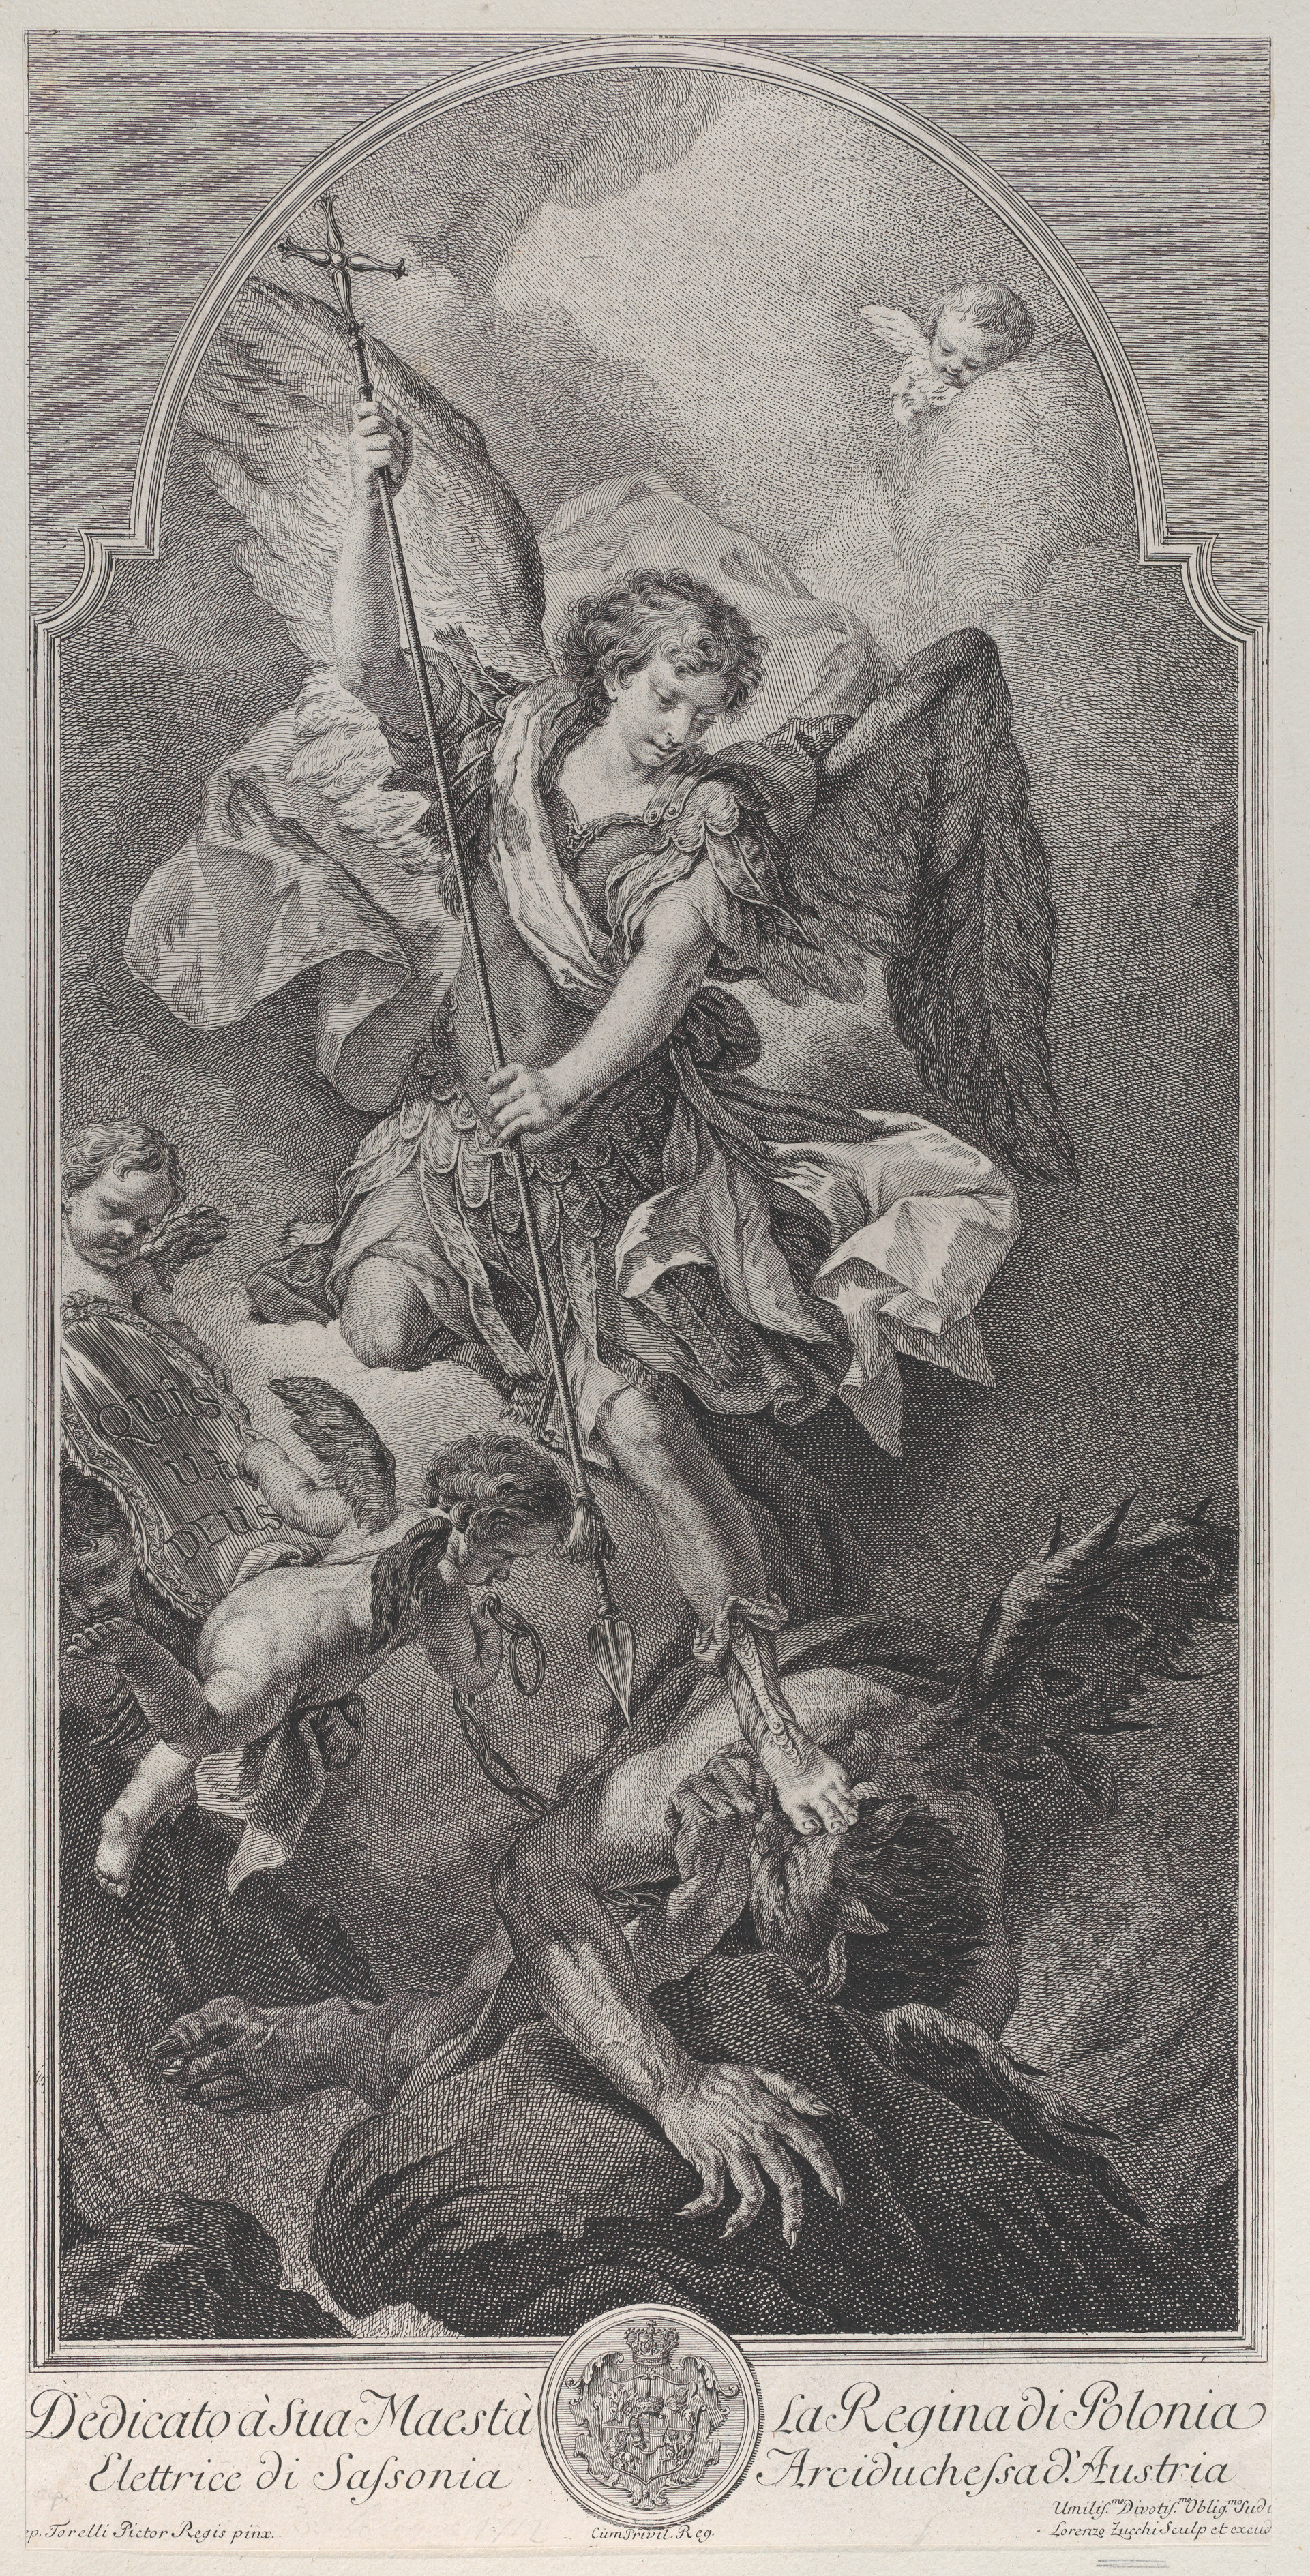
\includegraphics[height=0.75\textheight, keepaspectratio]{st_michael_defeating_satan.jpg}
	\caption{Saint Michael defeating Satan \cite{met_michael}}
	\label{fig:st_michael}
\end{figure}
\rubric{The Petition}

\begingroup
\centering
% LATIN
{\latinfont\Large
	Sáncte Míchael Archángele, defénde nos in proélio; \par
	contra nequítiam et insídias diáboli esto praesídium. \par
	Imperet illi Deus, súpplices deprecámur: \par
	tuque, Prínceps milítiae caeléstis, \par
	Sátanam aliósque spíritus malígnos, \par
	qui ad perditiónem animárum pervagántur in mundo, \par
	divína virtúte, in inférnum detrúde. \par
	Amen. \rubriccross \par
}

\vspace{1em}

% ENGLISH
{\itshape\small
	Saint Michael the Archangel, defend us in battle.
	Be our protection against the wickedness and snares of the devil;
	May God rebuke him, we humbly pray;
	and do thou, O Prince of the Heavenly Host, by the power of God,
	cast into hell Satan and all evil spirits
	who wander through the world for the ruin of souls.
	Amen. \par}
\endgroup

% ==========================================
% 4. THE LONG FORM EXORCISM
% ==========================================
\subsection{The Exorcismus in Satanam}
The long form exorcism prayer composed by Pope Leo XIII in 1890. This is reserved for use by bishops and authorized priests.

% --- MOVEMENT 1: THE INVOCATION ---
\rubric{The Invocation}
\textit{\small To be recited standing, with the Sign of the Cross made where indicated.}

\begingroup
\centering
% LATIN
{\latinfont\large
	In nómine Iesu Christi, Dei et Dómini nostri, \par
	intercessióne Immaculátæ Vírginis Dei Genetrícis Maríæ \rubriccross, \par
	Beáti Michaélis Archángeli \rubriccross, \par
	Beáti Ioánnis Baptístæ \rubriccross, \par
	Sanctórum Apostolórum Petri et Páuli \rubriccross, \par
	et ómnium Sanctórum, \par
	fidúcia ministérii nostri sacri, \par
	adversus versútias et insídias diáboli cum fidúcia aggredímur. \par}

\vspace{0.5em}

% ENGLISH
{\itshape\small
	In the Name of Jesus Christ, our God and Lord,
	strengthened by the intercession of the Immaculate Virgin Mary, Mother of God,
	of Blessed Michael the Archangel, of the Blessed Apostles Peter and Paul and all the Saints,
	and powerful in the holy authority of our ministry,
	we confidently undertake to repulse the attacks and deceits of the devil.\par}
\endgroup

\vspace{1.5em}

% --- MOVEMENT 2: THE PSALM (Psalm 67) ---
\rubric{Psalm 67 (Exsurgat Deus)}

\begingroup
\centering
{\latinfont\large
	Exsúrgat Deus, et dissipéntur inimíci eius: \par
	et fúgiant qui odérunt eum a fácie eius. \par
	Sicut déficit fumus defíciant; \par
	sicut fluit cera a fácie ígnis, \par
	sic péreant peccatóres a fácie Dei. \par}

\vspace{0.5em}

{\itshape\small
	God arises; His enemies are scattered and those who hate Him flee before Him.
	As smoke is driven away, so are they driven;
	as wax melts before the fire, so the wicked perish at the presence of God.\par}
\endgroup

\vspace{1.5em}

% --- MOVEMENT 3: THE COMMANDS ---
\rubric{The Commands}
\textit{\small The Exorcist commands the presence directly.}

\begingroup
\latinfont\large
\setlength{\parindent}{0pt}
\setlength{\parskip}{0.3em}

% Left-aligned (ragged right) for the 'Imperat' commands
Imperat tibi Deus Pater. \rubriccross \par
Imperat tibi Deus Fílius. \rubriccross \par
Imperat tibi Deus Spíritus Sanctus. \rubriccross \par
Imperat tibi Maiéstas Christi, Verbum Dei incarnátum. \rubriccross \par
Imperat tibi Virgo gloriósa, Dei Genetrix María. \rubriccross \par
Imperat tibi fides Sanctórum Apostolórum Petri et Páuli et aliórum Apostolórum. \rubriccross \par
Imperat tibi sanguis Mártyrum, imperat tibi pia intercessió Sanctorum et Sanctárum. \rubriccross \par
\endgroup

\vspace{0.5em}

\begin{quote}
	\itshape\small
	God the Father commands you.
	God the Son commands you. God the Holy Ghost commands you.
	Christ, God's Word made flesh, commands you.
	The glorious Mother of God, the Virgin Mary, commands you.
	The faith of the holy Apostles Peter and Paul, and of the other Apostles commands you.
	The blood of the Martyrs and the pious intercession of all the Saints command you.
\end{quote}

\vspace{1.5em}

% --- MOVEMENT 4: THE FINAL PRAYER (Missing Section) ---
\rubric{The Petition (Deus Caeli)}

\begingroup
\centering
{\latinfont\large
	Deus caeli, Deus terrae, \par
	Deus Angelórum, Deus Archangelórum, \par
	Deus qui potestátem habes donáre vitam post mortem, \par
	réquiem post labórem: \par
	quia non est Deus praeter te, \par
	nec esse potest nisi tu, Creátor ómnium visibílium et invisibílium, \par
	cuius regni non erit finis: \par
	humíliter maiestáti glóriae tuae supplicámus, \par
	ut omni potestáte infernálium spirítuum, \par
	ab ómnibus insídiis, decéptio, nequítia et furóre eórum, \par
	nos poténter liberáre, et incólumes custodíre dignéris. \par
	Per Christum Dóminum nostrum. Amen. \rubriccross \par}

\vspace{0.5em}

{\itshape\small
	God of heaven, God of earth, God of Angels, God of Archangels,
	God who has the power to give life after death and rest after work:
	because there is no other God beside Thee, nor can there be,
	Creator of all things visible and invisible, of whose kingdom there shall be no end:
	we humbly pray Thy glorious Majesty to powerfully deliver us
	from all the power, snares, deceits, wickedness, and fury of the infernal spirits,
	and to keep us safe and sound.
	Through Christ our Lord. Amen.\par}
\endgroup

\vspace{2em}
\hrule width 1.0\textwidth \relax
\vspace{2em}